% pme_theory.tex
%
% 19 March 01 am 
%	edited corrections into paper.
% 19 March 01 pm 
%	further corrections and references added. 
% 26 April 01 am
%	with corrections from Chris

% Post - defense corrections
% 29 May 2001
%	corrections from Chris
% 30 May 2001 corrections from Fred
% 30 may 2001 corrections from Paola
% 30 May 2001 corrections from R. Gomez

\chapter{A model of the paramagnetic Meissner effect 
in multiply-connected superconductors}
\label{chap:pme_theory}

\section{Introduction}

As discussed in  chapter \ref{chap:pme_experiment}, there have 
been many observations of PME in superconductors. 
In addition to these experimental observations, there 
have also been several theoretical attempts to explain 
the PME in these superconductors. 

\subsection[\pijunction\ models]{$\mathbf{\pi}$-junction models}

The first attempt to describe PME in \hightc\ superconductors came from
Sigrist and Rice \cite{sigrist_jpsj_61_4283_1992,%
sigrist_rmp_503_67_1995}, who argued that the presence 
of \pijunctions\ in a superconductor would cause it to be
paramagnetic. They further argued that \pijunctions\ would
come about due to a \dwave\ order parameter coupled with
misaligned grains in the superconductor. This idea is basically
the single loop model as discussed in chapter \ref{chap:jjarray}
(section \ref{sec:single_loop}, p. \pageref{sec:single_loop}, 
\EqnRef{eqn:steadystatepijunction}).
There we discussed at length that Sigrist and Rice was incomplete because they
 chose a value of 
\betal\ that was too small. Had they chosen a larger value
of \betal\ they would have seen that paramagnetism would be 
possible at zero external flux for a loop with no \pijunctions.
They attributed PME only  
to the presence of a \pijunction\ in the loop,
and hence evidence for \dwave\ superconductivity. 
Sigrist and Rice proposed this theory before the first
observation of PME in \lowtc\ superconductors
\cite{thompson_prl_75_529_1995}
and so were perhaps a bit overzealous in interpreting the implications.

\subsection{\jja\ models}

Since Sigrist and Rice based their work on the idea of a 
single superconducting loop, others began to try to model a
superconductor as various types of \jjas. One model, 
by Dominguez \etal\,\cite{dominguez_prl_72_2773_1994},
contained several flaws; they treat the case of a \jja\ with 
randomly distributed \pijunctions, but do not treat the case of an
array without \pijunctions, essentially repeating the mistake of 
Sigrist and Rice.
Dominguez \etal\ reached the similar conclusion that 
the presence of \pijunctions\ allows the sample to behave 
paramagnetically. 

Models of this
type were also studied by Auletta \etal\,\cite{auletta_prb_49_12311_1994}
who modeled the array as a series of concentric loops of \jjsnoun\  
including the mutual
inductance between the loops. 
Additionally, Chandran\,\cite{chandran_prb_56_6169_1997}
performed similar calculations using a square array and a full
mutual induction matrix. 
Both Auletta \etal\ and Chandran use 
simplified models for the \jjsnoun\
which ignore the capacitance of the
junction (RSJ model). 
Importantly, both treat only the case of \emph{no} \pijunctions, 
eliminating the problems with the Sigrist and Rice and the Dominguez \etal\
models. 
Remarkably, they were able to recreate the 
temperature-dependent magnetization during a model field cooling experiment
and show that it compares favorably with the 
previously reported experimental results (\cf\ Braunisch \etal\,
\cite{braunisch_prl_68_1908_1992,braunisch_prb_48_4030_1993}).
However, neither report on the spatial distribution of the
magnetization over the array, which we have directly measured
here. 

More recently, De Leo \etal\,\cite{deleo_unpublished}, used  
an RCSJ \jja\ to dynamically model the field-cooling process, and 
obtained results remarkably similar to the experimental results discussed in 
chapter \ref{chap:pme_experiment}. The relationship between this model
and the experiment will be discussed in more detail in section
\ref{sec:num_array_sims}. 

\subsection{Flux compression}

In a departure from the \jja\ model of PME,
Koshelev and Larkin \cite{koshelev_prb_53_13559_1995}
proposed the flux compression model. \index{flux compression}
The flux compression model relies on the superconductor having a 
spatial variation in \tc, such that the exterior of the sample
becomes superconducting before the interior of the sample.
Because the exterior becomes superconducting first, it 
effectively traps flux in the center of the sample, and compresses
the trapped flux (hence ``flux compression'') as the 
superconducting region grows
from the outside-in. This trapped flux, and the
screening currents required to keep the flux trapped, create
a positive magnetic moment, the paramagnetic Meissner effect.
An important aspect of the flux compression model is that it gives
specific predictions for the flux and current distribution
throughout the sample -- something that can easily be tested with
the SQUID microscope. 

A phenomena related to the flux compression model is the ``giant
vortex state'' model\,\cite{moshchalkov_prb_55_11793_1999,%
deo_prl_79_4653_1997}. It may be appropriate for mesoscopic
superconductors, such as the aluminum disks measured by Geim \etal\
\cite{geim_nature_396_144_1998}, but does not apply to the 
macroscopic situations discussed here. 

\subsection{Pinning and surface barriers}

In addition there are other proposed models which essentially rely
on defects in the superconductor to create the PME. 
One may imagine, \eg\, that surface damage to the superconductor
pins flux during the field cooling process 
and causes the sample to be paramagnetic. It has
additionally been proposed that some type of surface barrier
may result in flux trapping in the sample \cite{deo_prb_59_6039_1999},
or that 
Andreev bound states at the
surface of the superconductor \cite{prusseit_physc_317_396_1999}
may result in paramagnetism. 

\section{Comparison of experimental data to various models}

Simple models involving \pijunctions\ do not apply to the niobium 
\jja\ samples that were measured. 
It has clearly been demonstrated that niobium, an \swave\ superconductor,
exhibits PME in the absence of \pijunctions. Furthermore, it is
clear from the discussion of the single loop in chapter \ref{chap:jjarray}\
that a single loop of \jjsnoun, without any \pijunctions, can in
theory be paramagnetic after field cooling. 

The various \jjnoun\ models treating PME in an array model of 
superconductivity
have great merit, but do not provide any spatially resolved data
to which we might compare our array data. Additionally, we 
cannot practically measure the sample magnetization \vs\
temperature during the field cooling process, in order to 
compare with their models. In order to do this we would
need to stop and image the array many different times as we cool
it through \tc\ to $4.2\,\kelvin$. In principle we can do this, 
but we cannot maintain temperature stability near \tc\ in order 
for these scans to be more interesting than the scans presented
herein. However, the spatially resolved data we obtain is 
extremely useful for the comparison with many of these theories, 
and, as we will show, motivates our explanation for the 
phenomena of PME.

Based on our experimental observations we can clearly rule out
the flux compression model as untenable. Our data looks nothing
like the proposed flux distribution for a sample exhibiting
flux compression and in fact looks quite random. 
This is really not surprising since
we do not expect any of the 
requirements of flux compression to be met in our experiment. 
First, our sample is well grounded thermally to the sapphire rod of the
sample stage in the experiment. Furthermore, because of the
photolithographic uniformity
we do not expect that the outermost islands of the 
array would have a \tc\ \emph{higher} than the inner islands.
In fact in our arrays, we expect there to be no preference for
deposition errors near the edges. However, in thin film samples
we might expect  
deposition errors to cause the sample edge 
to have defects
which would tend to 
\emph{lower} the sample \tc. 

Indeed, the primary features of our experimental data are not
predicted by any of the published theories of PME. We always observe a
diamagnetic region around the edge of the sample in addition to 
a region of Gaussian distributed flux inside, but generally with
a  paramagnetic mean. Finally, the paramagnetism of the array appears to 
increase
with increasing external field. 

\section{Mean field theory of \jja}

\index{mean field theory}
A very simple approximation is to assume that each loop
in the \jja\ behaves identically, and sees a mean field due to the
response of the other loops in the array. 
This may be expressed as 
%
\begin{equation}
\label{eqn:meanfield}
-(\phitot-\phiext) = \left. \frac{\dif G}{\dif\phiext}\right|_{\phiext + \lambda
(\phitot-\phiext)}
\end{equation}
% 
where the coupling parameter $\lambda = {\sum \atop {i\ne j}} M_{i,j}/L$, 
and $M_{i,j}$ is the mutual inductance matrix. In practice, the summation
must be cut off at the physical size of the array considered. We solved 
\EqnRef{eqn:meanfield} numerically and found that the a paramagnetic array
actually has its paramagnetism \emph{enhanced} slightly by the 
mean field. Conversely, a diamagnetic array becomes more diamagnetic
under the influence of the mean field. \FigRef{fig:mean_field} shows the
effect of this mean field on the array magnetization. The figure 
shows the magnetization of a simple single loop (solid line) and
the magnetization of a single loop under the influence of the 
mean field (dashed line) from which it's clear that the magnetization of the
loop is enhanced a small mount under the influence of the mean 
field.

The mean field model thus fails to agree with \FigRef{fig:sm_array_mag_plot} 
and 
\FigRef{fig:lg_mag_vs_ext}
which show a preference for paramagnetic response.

%
% mean field theory plot 
%
\begin{figure}[p]
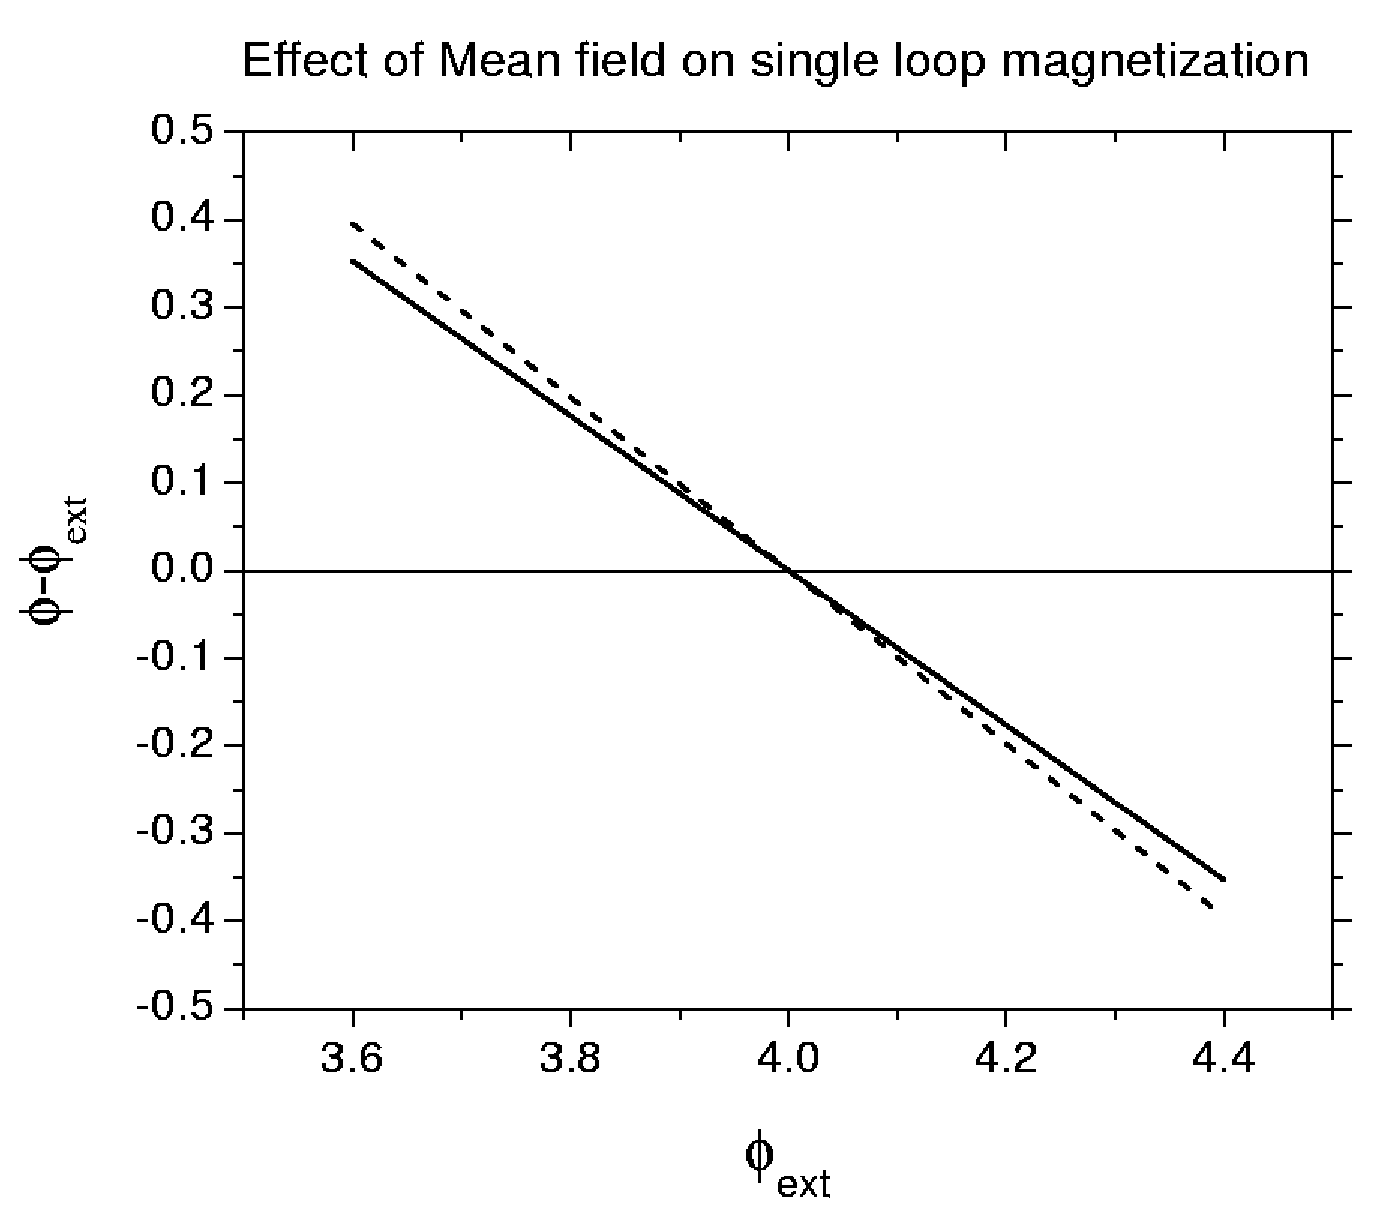
\includegraphics[width=5.7in]{figs/jjarray/chap2fig7.eps}
\caption[Effect of the mean field due to surrounding plaquettes in the array.]
{Effect of the mean field due to the surrounding plaquettes in the array on
a given test plaquette. Plaquette magnetization plotted \vs\ \phiext\
for the case of a single loop without the mean field (solid line) and
the case of the single loop in the presence of the mean field (dashed line).}
\label{fig:mean_field}
\end{figure}

\section{Array screening}

The presence of the diamagnetic screening current flowing around
the outside edge of the array must be accounted for in any 
realistic model. The array could accomplish this diamagnetic
screening in one of two ways. 

\begin{figure}[p]
\includegraphics[width=5.7in]{figs/pme_theory/fig41.eps}
\caption[Comparative array screening: individual plaquette \vs\ 
large outside loop.]
{Different ways to generate Meissner screening in an array.
(a) A large loop of many \jjsnoun\ around the outside edge of the
array. (b) Each plaquette screens flux from the its own interior,
and hence screening flux from the entire array. }
\label{fig:comp_array_screening}
\end{figure}

First, the array, of size $N\times M$, may generate a screening
current flowing around the outside edge of the array
(large loop screening); in effect
creating a large loop of $2(N + M)$ junctions around the outside
of the array. 
\MultFigRef{fig:comp_array_screening}{a}\ depicts this situation. 
This picture is similar to how a bulk 
superconductor might screen, with current flowing just around the outside
edge and nowhere else inside. 
We want to know the maximum external field that this 
large loop can screen. To do this, we need to know how the self
inductance of a square grows as the wire size grows. 

\subsection{Self-inductance of square loop}
\label{sec:self_ind_square_loop}
\index{self inductance!square|(emph}

The self-inductance of a current loop
may be defined from\footnote{See Landau and Lifshitz\cite{landau_lifshitz_em},
pp.~136-139
for an excellent discussion of the self inductance.
They reach similar conclusions as to those drawn here.}
%
\begin{equation}
L I = \Phi
\label{eqn:self_ind_defn}
\end{equation}
%
in which $\Phi$ is the flux induced in the current loop due to the
current $I$ and $L$ is the self-inductance.

A straightforward approach to the calculation of the self-inductance
of a square loop is to determine the flux via the vector 
potential
$\vec{A}(\vec{x})$ which is determined from the 
current flowing around the loop.
For a square loop it is convenient to 
discretize the loop into four wires (each side of the square) and
compute the vector potential due to each wire segment. With the vector
potential we
compute the flux using
%
\begin{equation}
\Phi = \oint \vec{A}\cdot\,\dif \ell 
\label{eqn:flux_vec_pot}
\end{equation}
%
around the entire square. 
The geometry for this calculation is shown schematically in 
\FigRef{fig:self_ind_geometry}.

\begin{figure}[p]
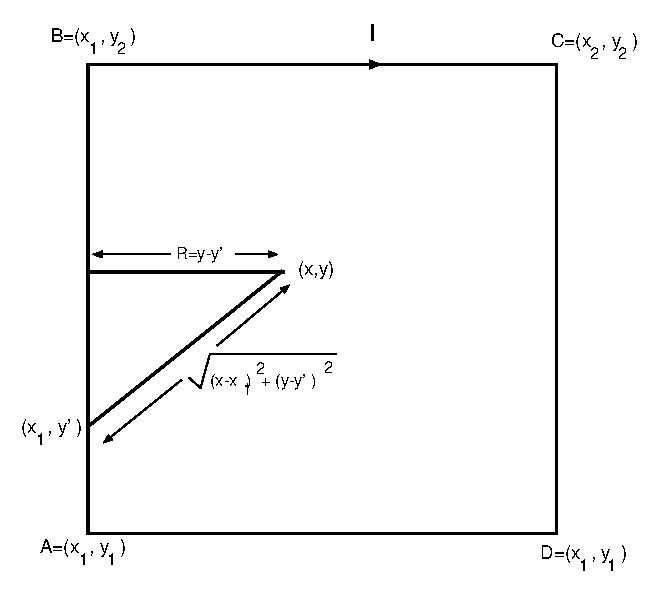
\includegraphics{figs/pme_theory/selfindgeom.eps}
\caption[Geometry for calculation of square loop self inductance.]
{Geometry for calculation of square loop self inductance. The half width of 
the wire $W$ is not shown here, and is taken as much smaller than the 
distance between any of the vertices of the square, \ie\ 
$W\ll \left|y_2 - y_1\right|$. }
\label{fig:self_ind_geometry}
\end{figure}

The vector potential for a current distribution may be determined from%
\footnote{This derives from Maxwell's equations and the definition of the
vector potential $\vec{B}=
\nabla \times \vec{A}$. See Jackson\cite{jackson},
pp. 173-176 for a complete discussion of the derivation.
This form implies the choice of the Coulomb gauge, 
$\nabla \cdot \vec{A}=0$.}
%
\begin{equation}
\vec{A}(\vec{x}) = {\mu_0 \over 4\pi} \int_V {\vec{J}(\vec{x})\over
\left|\vec{x}-\vec{x}'\right|} \dif^3 \vec{x}'
\label{eqn:vec_pot_a}
\end{equation}
%
in which $\vec{J}(\vec{x})$ is the current density distribution
and $V$ is over the entire volume of the current density.
We assume that the current density distribution is small in extent
and may be treated as a constant
so that \EqnRef{eqn:vec_pot_a} may be reduced to 
%
\begin{equation}
\vec{A}(\vec{x}) = {\mu_0 I  \over 4\pi}\oint {\dif\ell'\over 
\left|\vec{x}-\vec{x}'\right|}.
\label{eqn:vec_pot_b}
\end{equation}
%
If we consider the vector potential due to one single side of the 
square, $\overline{AB}$, in \FigRef{fig:self_ind_geometry}, the
integration in \EqnRef{eqn:vec_pot_b} becomes
%
\begin{equation}
\vec{A}(x,y) = {\mu_0 I \over 4\pi} \hat{y} \int_{y_1}^{y_2}\,
{\dif y' \over \sqrt{(x-x_1)^2+(y-y')^2}}.
\end{equation}
%
This integrates to become
%
\begin{equation}
A_y(x,y) = {\mu_0 I  \over 4\pi} \left\{\sinh^{-1}\left(\frac{y-y_2}{x-x_1}\right) - \sinh^{-1}\left(\frac{y-y_1}{x-x_1}\right)\right\}.
\label{eqn:vec_pot_sinh}
\end{equation}
We have implicitly assumed that the point $(x,y)$ in 
\EqnRef{eqn:vec_pot_sinh} is outside of the wire. If we define
the halfwidth (or radius) of the wire to be $W$ this implies that
$W\ll \left|y_2 - y_1\right|$.
Similarly we can compute the vector potential due to each of 
the remaining three wire segments of the square. With these
four components to the vector potential we may compute total flux 
due to the current numerically through \EqnRef{eqn:flux_vec_pot} and
the self inductance through \EqnRef{eqn:self_ind_defn}.

We expect the self inductance to go to zero as the area of the loop goes
to zero in this model. However, in the limit of zero area, the model
described here is no longer valid. Instead, see Jaycox and Ketchen
\cite{jaycox_ieeetm_mag17_400_1981} for a discussion of the 
self inductance of a finite width wire loop. 

We expect
that as the loop grows arbitrarily large, the self inductance will
grow linearly. In this limit, we can neglect the finite size of the
wire width making up the square and use Ampere's Law to simply 
compute the magnetic induction due to the current as
%
\begin{equation}
B(r) = {\mu_0 \over 2 \pi} {I \over r},
\end{equation}
$r$ being the distance from the wire. Furthermore, the area
of the square grows like $r^2$. Therefore the self-inductance
grows like
%
\begin{equation}
L I \propto B A \propto {1 \over r} r^2 = r
\end{equation}
%
or linearly with the size of the square. When we compute the self
inductance numerically, this is exactly the dependence we find.
The computed self inductance is 
plotted in \FigRef{fig:self_ind_plot} for a range of square sizes
similar to our overall array size.

%
% self inductance of square loop versus loop size
%
\begin{figure}[p]
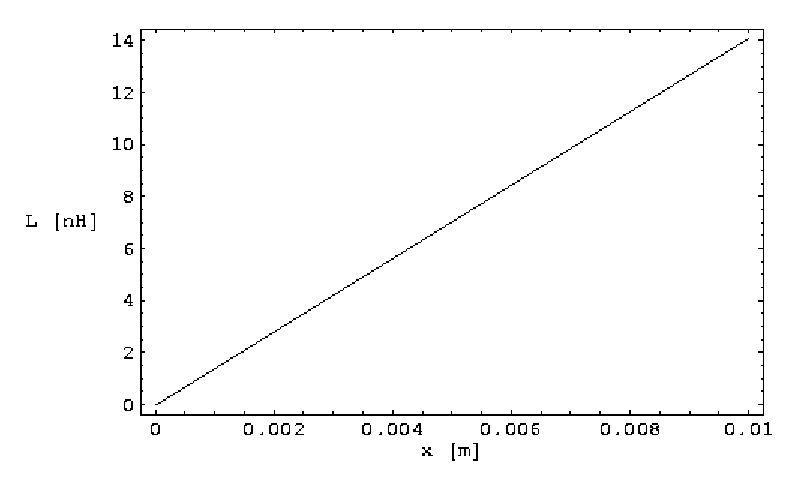
\includegraphics[width=5.7in]{figs/pme_theory/squareselfinductance.ps}
\caption[Computed self inductance of a square current loop.]
{Computed self inductance of a square current loop.}
\label{fig:self_ind_plot}
\end{figure}

\index{self inductance!square|)}


\subsection{Screening due to large loop around edge of array}

A single plaquette may screen flux from 
itself up to\footnote{Recall, from \EqnRef{eqn:dimensionless_subs}, 
that $\betal = 2 \pi L I_c / \Phinot$ in which 
$L$ is the self inductance of a single plaquette and $I_c$ is 
the critical current of a single junction.}
%
\begin{equation}
B_{\mathrm{max}} = \Phinot \betal /2 \pi a^2
\label{eqn:single_array_max_flux}
\end{equation}
%
In the previous section we discussed how the self inductance 
of a square loop grows linearly with the size of the loop.
Because of this linear dependence on \betal\ a  
large current loop around a $M\times N$ array  
can screen a maximum external field of 
%
\begin{equation}
B_{\mathrm{max}}={\Phinot \betal \over 2 \pi a^2 (NM)^{1/2} } \mbox{,}
\end{equation}
%
which assumes that $M\approx N$.

\subsection{Screening due to single plaquettes}

The second possibility for screening in the array 
is that each individual plaq\-uette 
screens flux from 
itself. As mentioned above, the maximum external field 
screened from a single plaquette is
%
\begin{equation}
B_{\mathrm{max}} = \Phinot \betal /2 \pi a^2. 
\end{equation}
%
In this picture, flux will not penetrate the array until flux
is able to penetrate a single plaquette. The maximum
field in this case is always greater, and substantially greater
for extremely large arrays than the maximum flux of
\EqnRef{eqn:single_array_max_flux}, making this difference
quite easy to discern experimentally. 
There are two ways to think of the screening in this case. 
Both of these are shown in \FigRef{fig:plaquette_screening}. 

\begin{figure}[p]
\includegraphics[width=5.7in]{figs/pme_theory/fig43.eps}
\caption[Different array screening configurations for individual
plaquettes.]
{Possible different array screening configurations. (a) Every
plaquette of the array screening. (b) Only the outside edge plaquettes
of the array screening. }
\label{fig:plaquette_screening}
\end{figure}

In \MultFigRef{fig:plaquette_screening}{a}\ each plaquette of the array
sets up a screening current to shield out the external flux. 
One might assume that the opposing currents internal to the array
will cancel, reducing this case to the large loop case shown in
\FigRef{fig:comp_array_screening}. However, there is a 
crucial distinction
to be made. The current is flowing in niobium wires of 
width $10\,\micron$, but niobium has a London penetration depth of
$900\,\angstrom$ at $4.2\,\kelvin$. \FigRef{fig:plaquette_screening_close_up}
shows this situation schematically for two adjacent plaquettes. 
The screening current for one plaquette does not cancel the 
screening current for the adjacent plaquette because the screening
currents are flowing only within the penetration depth, and there is
no physical overlap between the two currents. 

\begin{figure}[p]
\includegraphics[width=5.0in]{figs/pme_theory/fig44.eps}
\caption[Close up view to two adjacent plaquettes with screening 
currents.]
{Close up view of two adjacent plaquettes with screening currents. 
The geometry
is for our experimental array. 
The wire width is $10\,\micron$ and the penetration
depth for niobium is $900\,\angstrom$. Because of the difference
of the length scales,
the internal currents (indicated by the arrows) 
do not cancel, and the array
must actually generate a loop of current flowing around each
plaquette}
\label{fig:plaquette_screening_close_up}
\end{figure}

%In \MultFigRef{fig:plaqutte_screening}{b}\ only the outside plaquettes
%of the array generate the screening current. Again, opposing currents
%do not cancel for the reasons discussed above.

%One helpful way to think about these two configurations is to realize 
%that in both cases, the maximum current that may flow around any 
%current path is the critical current, $I_c$. 
%Presented here are the two limiting cases. 
%In the large loop current case, the maximum field is screened when
%$I_c$ flows around the entire array. In the second case, the maximum
%flux may be screened when $I_c$ flows around a single plaquette. 
%It is clear that the amount of flux that flows through the enclosed
%area, due to the currents, is far larger in the latter case than
%in the former. 

AC susceptibility measurements by Araujo-Moreira \etal
\cite{araujo_prl_78_4625_1997} demonstrated the 
distinction between large loop screening and single plaquette
screening and showed that the arrays generate single plaquette
screening.
They showed that 
the array did not respond hysteretically to a driving external field
until the amplitude of the external field was increased above approximately
four flux quanta per unit cell. For the $\betal =30 $ used here this
indicates that single
plaquettes of the array are screening.  
Furthermore, we have observed the onset of 
flux penetration into our array, initially in the
Meissner state, and noticed that the flux does not penetrate until the
external field is ramped from zero to exceed two to 
four flux quanta per unit cell
of the array. By contrast, \EqnRef{eqn:single_array_max_flux} predicts
$\Phi_{\mathrm{max}}=0.09\,\Phinot$ per unit cell. 

%An example of this penetration is shown in 
%\FigRef{fig:init_flux_penetration}. The figure shows the first
%flux penetration into the array at a field of $4.8\,\Phinot$ per unit cell 
%of the array. Notice that the flux penetrates as fingers, apparently
%nucleating from a single plaquette, indicating that it was the screening
%of a single plaquette that broke down (perhaps due to a locally lower 
%critical current) 
%and allowed flux to penetrate. 

%\begin{figure}
%\includegraphics[clip=true]{figs/pme_theory/fig42.eps}
%\caption[Initial flux penetration into \jja]{Initial flux 
%penetration into \jja\ at an external field of 4.8 \Phinot
%per unit cell.}
%\label{fig:init_flux_penetration}
%\end{figure}

\subsection{Outer diamagnetic current}

The previous section presented evidence that the array
screens flux using the single plaquette screening model, as
distinct from the large loop screening model. 
We observed 
(\cf\ \FigRef{fig:paramag_image_a} and \FigRef{fig:paramag_image_c}
in all of the 
field-cooling images that the array always generated a diamagnetic 
screening current around the outside edge. To
generate an overall diamagnetic screening current,
and have each plaquette screen individually, one may initially think
that the array behaves as is shown schematically in
\MultFigRef{fig:plaquette_screening}{a}. We discussed previously how
the currents do not cancel in this model. However, the currents 
are confined within the wires, which are $10\,\micron$ wide, and we
cannot resolve features smaller than about $50\,\micron$ so we cannot
identify these currents internal to the array. 


% currents canceling in overlap geometry junctions. 
%
% need reference for this
%
%We argued above that 
%the internal currents to the array do not cancel within the wires. 
%It turns out that in the overlap \jjnoun\ geometry the current
%flowing through the \jjnoun\ spreads out uniformly so we expect
%the currents flowing through the junctions to cancel, and not
%give a contribution to the net Josephson energy. 

To generate the configuration in
\MultFigRef{fig:plaquette_screening}{a}\ we find that the energy stored
magnetically due to all the plaquette current loops in the array 
is
%
\begin{equation}
E_{\mathrm{mag}} = NM\, \frac{1}{2} LI^2.
\end{equation}
%
Additionally, there is a Josephson energy contribution to the energy
from the junctions around the outside edge of the array
%
\begin{equation}
E_{J \mathrm{tot}} = 2(M+N)\, E_J (1-\cos\gamma)\mbox{,}
\end{equation}
%
in which $E_J=\hbar I_c/2 e$ is the Josephson coupling energy of the junction
(note that the currents through the junctions cancel while the currents in
the wires do not).
This leads to a total energy of 
%
\begin{equation}
E_{\mathrm{tot}} =  NM \,\frac{1}{2} LI^2 + 
          2(M+N)\, E_J (1-\cos\gamma).
\label{eqn:all_loop_screening}
\end{equation}
%
This total energy grows as $N\times M$, and for a large array can be quite 
substantial. 

It turns out that it is possible to screen while having the total
energy grow as $N+M$. 
This screening configuration is shown in 
\MultFigRef{fig:plaquette_screening}{b}. Here only the plaquettes on 
the outside edge of the array screen. This creates the observed external
diamagnetic screening current. But we end up with a total magnetic
energy of 
%
\begin{equation}
E_{\mathrm{mag}} = 2(N+M)\, \frac{1}{2} LI^2.
\end{equation}
% 
Additionally, there is a contribution due to the Josephson energy
in the outside edge junctions, and also from the edge 
junctions just inside the screening plaquettes, as shown in 
\MultFigRef{fig:plaquette_screening}{b}. 

In the inside edge junctions
%
\begin{equation}
E_{J \mathrm{tot}} 
=\left\{ 2(N+M) + 2(N + M - 2) \right\}\, E_J (1-\cos\gamma),
\end{equation}
%
yielding a total energy of 
%
\begin{equation}
E_{\mathrm{tot}} = 2(N+M)\, \frac{1}{2} LI^2 +
 \left\{ 2(N+M) + 2(N + M - 2) \right\}\, E_J (1-\cos\gamma).
\label{eqn:edge_loop_screening}
\end{equation}
%
This energy is smaller than the energy in the previous case,
\EqnRef{eqn:all_loop_screening},
in which all of the plaquettes screen. As the size of the array
grows, this energy becomes more favorable (\cf\ $N+M$ \vs\ $N\times M$).

Comparing \EqnRef{eqn:all_loop_screening}\ and 
\EqnRef{eqn:edge_loop_screening}\ with the assumption
that the gauge invariant phase difference is 
proportional to the total flux and that the array is square (\ie\ $N=M$)
we deduce that it will be energetically
favorable for the array to screen with only the outside
edge plaquettes when
%
\begin{equation}
\betal > {4 N -1 \over N^2 - 4N}\mbox{,}
\end{equation}
%
valid for all $N>2$. For the arrays we consider, this 
criteria is easily satisfied. 

\section{Consequences of edge loop screening}

In the case shown in \MultFigRef{fig:plaquette_screening}{b}, 
with only the edge loops screening, 
in addition to the diamagnetic screening current flowing immediately
around the outside edge, there also is a paramagnetic
current flowing just inside the outside edge. This paramagnetic
current is closer to the interior of the array than the diamagnetic
current. The interior plaquettes of the array will respond to both
the diamagnetic current and the paramagnetic current, but the 
paramagnetic current is closer to the interior plaquettes, so 
it will dominate the response of the interior plaquettes. 
\FigRef{fig:screening_schematic}\  schematically shows this situation, 
depicting the external diamagnetic screening current and the interior
paramagnetic current.

\begin{figure}[p]
\includegraphics[width=5.7in]{figs/pme_theory/fig45.eps}
\caption[Schematic of interior and exterior plaquettes, with screening
provided by external plaquettes only.]
{Schematic of interior and exterior plaquettes, with screening provided
by external plaquettes only. The diamagnetic screening current flows 
around the outside edge of the array, while the paramagnetic current
flows just inside the edge of the array.}
\label{fig:screening_schematic}
\end{figure}

\subsection{Internal plaquette response to fields generated by external
plaquettes}

Simplistically 
each interior plaquette sees a field made up of the external field
applied to it plus fields due to the diamagnetic and paramagnetic currents
discussed above. 
The external flux
that each interior plaquette sees is the real external flux, 
plus a flux contribution due to the edge plaquette currents,
$\Phi_{\mathrm{screen}}$.
If we analyze the interior plaquettes as single loops 
(chapter \ref{chap:jjarray}) the external flux we need to use
is slightly modified
%
\begin{equation}
\Phiext \rightarrow \Phiext + \Phi_{\mathrm{screen}}.
\label{eqn:ext_flux_redef}
\end{equation}
%
If we apply this modification to the magnetization relation for a 
single loop, shown in \FigRef{fig:single_loop_mag}, we see that the
entire magnetization curve for the single loop is shifted upward
so that the single loop will more often be 
\emph{paramagnetic}. 
%It must be pointed out here that this 
%shift is really just a book-keeping shift, because of the 
%redefinition of the external flux that affects the single 
%loop, \EqnRef{eqn:ext_flux_redef}. 

\subsection{Array response to external field plus screening fields}

We computed the screening flux
over the entire interior of the array
of the $30 \times 100$ array and
determined the shift in the magnetization of each interior
plaquette. We found that the 
minimum induced magnetization occurs in the central plaquette of
the array and is approximately $\Phimag=0.15\,\Phinot$. Furthermore,
we determined the average induced magnetization over the 
entire interior of the array, and determine it to be 
$\langle\Phimag\rangle=0.27\,\Phinot$. 
These numbers compare favorably with the observed
average
magnetization numbers seen in the array (\cf\ \FigRef{fig:sm_array_mag_plot}).

Of course, this simple model does not capture many other important
features experimentally observed in the array. It does not explain
\eg\ the apparent random distribution of flux over the interior of the
array. Quite the contrary, it predicts that the paramagnetism should
be strongest near the edges of the array, and weakest in the center
of the array. Furthermore, this simple model predicts that the array
interior
should be entirely paramagnetic while we observe that there
are diamagnetic regions in the array interior. 
The ingredient missing from the simple model is that all
the plaquettes influence each other -- it is too simple to assume
that only the edge plaquettes influence the interior ones. 

\subsection{Numerical array simulations}
\label{sec:num_array_sims}

Numerical simulations of an array system,
with no \pijunctions, similar to ours,
using the RCSJ model for the entire array (\cf\ chapter \ref{chap:jjarray},
section \ref{sec:entire_array_model}, p.~\pageref{sec:entire_array_model}
and  Eqns.~(\ref{eqn:junc_horiz}) to 
(\ref{eqn:total_flux_array})) have been carried out recently
\cite{deleo_unpublished} and yield results that replicate quite
well the experimentally observed flux distribution in the array.

In this simulation, De Leo \etal\ take a $10\times 40$ 
\jja\ and model the experiment by increasing in small steps
%
\begin{equation}
\betal= {2 \pi \over \Phinot} L I_c(T) 
\end{equation}
%
and
%
\begin{equation}
\betac= {2 \pi \over \Phinot} I_c(T) R^2  C 
\end{equation}
%
from zero at \tc\ to their final values at $T=4.2\,\kelvin$.
By holding all the parameters constant except for $I_c$ this
amounts to increasing $I_c$ as the temperature decreases.
For the resistance $R$ of the junction we chose the sub
gap resistance, which gives a value of $\betac = 66$ at 
$4.2\,\kelvin$. The material parameters for our \jja\ samples
were discussed in section~\ref{sec:sample_description},
p.~\pageref{sec:sample_description} and we also used
$\betal=30$ at $4.2\,\kelvin$.

\begin{figure}[p]
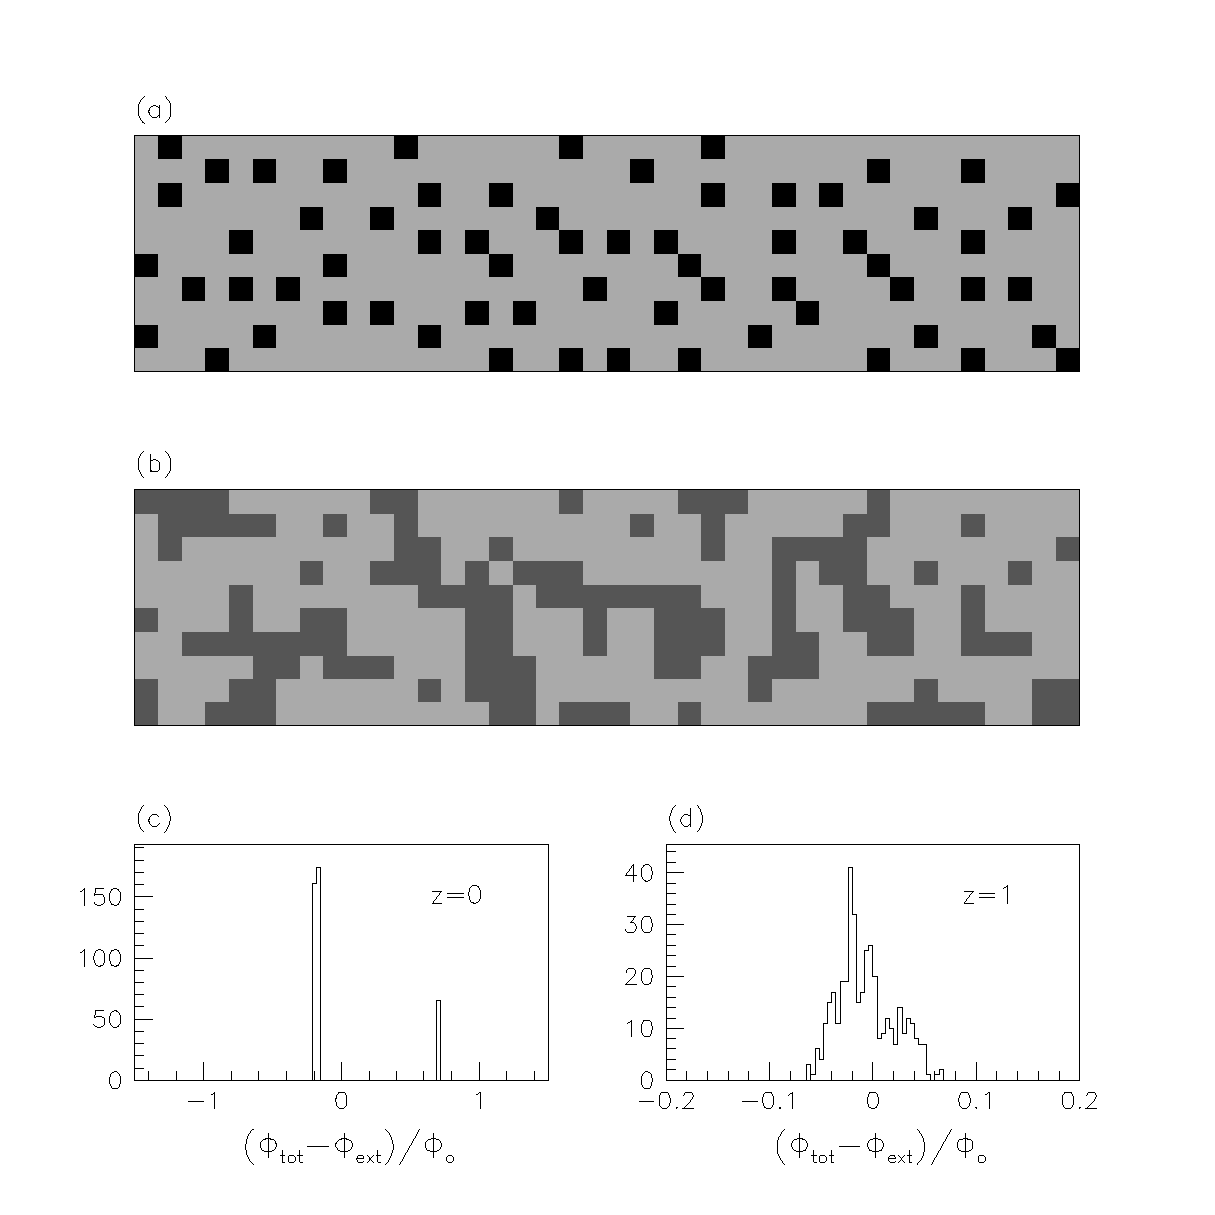
\includegraphics[width=5.7in]{figs/pme_theory/fig46.eps}
\caption[Modeled array magnetization for a $10\times 40$ \jja,
field cooled in $\phiext = 4.8$.]
{Modeled array magnetization for a $10\times 40$ \jja, field
cooled in $\phiext = 4.8$. 
Dark grey represents paramagnetic plaquettes and light grey represents
diamagnetic plaquettes.
(a) The array magnetization at the surface of the array. 
(b) The array magnetization as measured at a height of one
unit cell above the array. 
(c) Histogram of the array magnetization at the surface of the
array.
(d) Histogram of the array magnetization at a height of one
unit cell above the array. }
\label{fig:model_array_mag}
\end{figure}

\FigRef{fig:model_array_mag}\ shows the results of a field
cooling simulation for a $10 \times 40 $ \jja. Dark grey represents
paramagnetic plaquettes and light grey represents diamagnetic 
plaquettes. \MultFigRef{fig:model_array_mag}{a}\ shows the 
magnetization as measured at the surface of the array, and
\MultFigRef{fig:model_array_mag}{c}\ shows a histogram of the
same data. The spatial distribution of the magnetization in (a)
is very suggestive of the data we measured (\cf\ 
\FigRef{fig:paramag_image_a} and \FigRef{fig:paramag_image_c}). 
However, the histogram in 
\MultFigRef{fig:model_array_mag}{c} is quite different from that
measured in \FigRef{fig:paramag_image_b}. What's truly
striking about  \MultFigRef{fig:paramag_image_b}\ however, is that
the two peaks correspond almost exactly to the lowest and second
lowest Gibbs free energy solutions for the single loop
(\cf\ chapter \ref{chap:jjarray}, section \ref{sec:gibbs_free_energy},
p. \pageref{sec:gibbs_free_energy}). 

Perhaps more interesting,
\MultFigRef{fig:model_array_mag}{b}\  shows the simulated
magnetization of the $10 \times 40 $ array at a height of one 
plaquette. This is similar to the magnetization that a SQUID might
measure at a height of one plaquette. Indeed the SQUID in our 
experiments was at a height of approximately one plaquette. 
Interestingly, the histogram shown in \MultFigRef{fig:model_array_mag}{d}\
closely resembles the experimental histogram in 
\MultFigRef{fig:paramag_image_d}.

Furthermore, De Leo \etal\ modeled the external field dependence of the 
array magnetization, shown in \FigRef{fig:sim_array_mag}. Their results
qualitatively resemble the results obtained in \FigRef{fig:sm_array_mag_plot},
providing good evidence that the properties of our array can be replicated
simply from the equations describing a \jja, without \pijunctions. 

%
%  array mag per cooling field
%
\begin{figure}
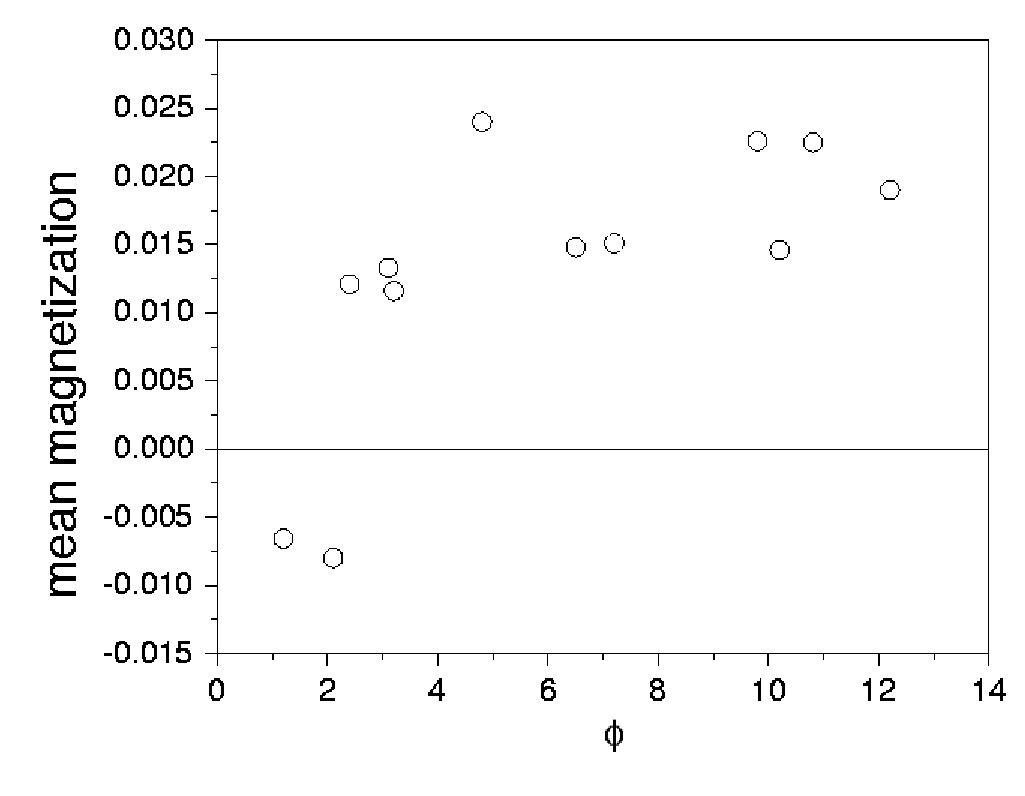
\includegraphics[width=5.7in]{figs/pme_theory/fig47.ps}
\caption[Simulated array magnetization \vs\ cooling field.]
{Simulated array magnetization \vs\ cooling field for the 
$10\times 40 $ \jja. The frustration is {\Phiext/\Phinot} per
unit cell of the array, and the mean magnetization is 
$\langle \Phimag / \Phinot \rangle$ per unit cell of the array.}
\label{fig:sim_array_mag}
\end{figure}
